\newSection{Motivation}

%---------------------------------------------------------
\begin{frame}[t]{Motivation}
    \textbf{Main Challenge:} Using synthetic data as a prior for real-world 3D hair modeling introduces a domain gap.
\end{frame}

%---------------------------------------------------------
\begin{frame}[t]{Motivation}
    \textbf{Main Challenge:} Using synthetic data as a prior for real-world 3D hair modeling introduces a domain gap.

    \vspace{1em}
    \textbf{Existing Solutions:} 
    \begin{itemize}
        \item Utilize undirected 2D orientation maps as an intermediate representation between the input image and the 3D hair model.
    \end{itemize}
\end{frame}

%---------------------------------------------------------
\begin{frame}[t]{Motivation}
    \textbf{Main Challenge:} Using synthetic data as a prior for real-world 3D hair modeling introduces a domain gap.

    \vspace{1em}
    \textbf{Existing Solutions:} 
    \begin{itemize}
        \item Utilize undirected 2D orientation maps as an intermediate representation between the input image and the 3D hair model.
    \end{itemize}

    \vspace{1em}
    \textbf{Limitations:}
    \begin{itemize}
        \item Ambiguous directionality: Loses 3D cues from the image.
        \item Reliance on image filters: Adds noise and inaccuracies.
    \end{itemize}
\end{frame}

%---------------------------------------------------------
\begin{frame}[t]{Motivation -- Visualization}
    \begin{figure}[t]
        \centering
        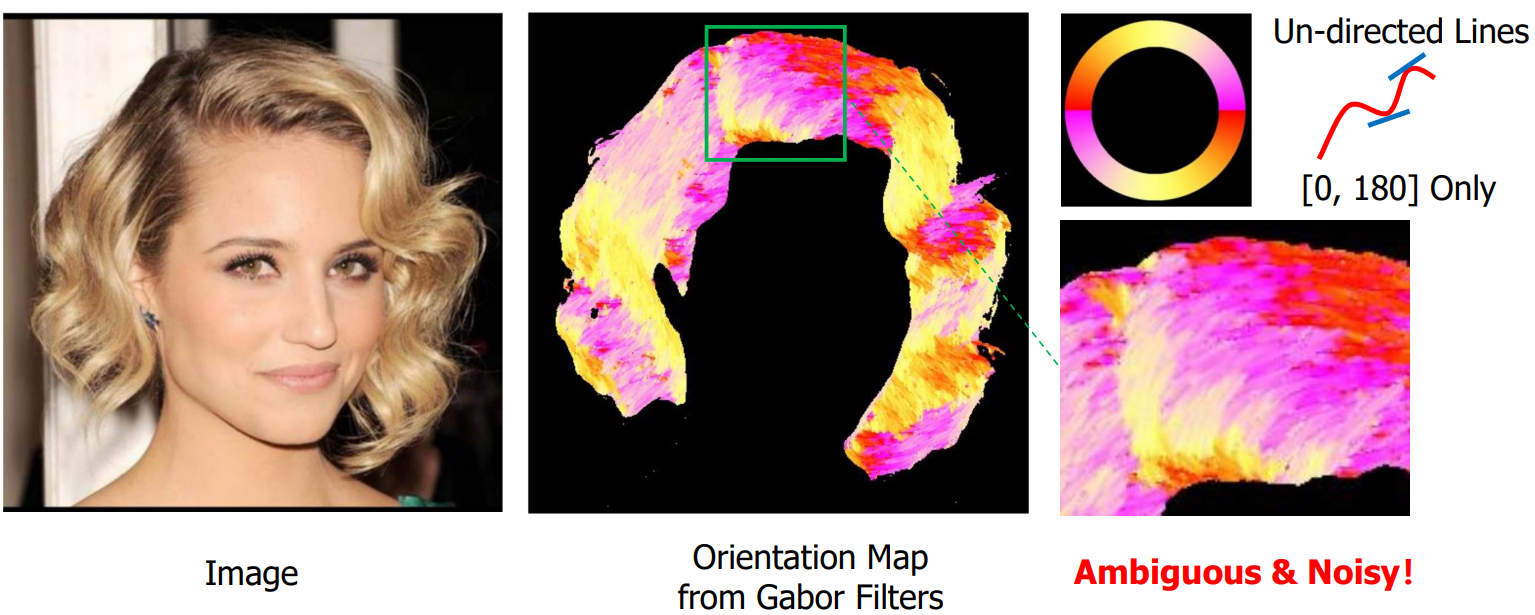
\includegraphics[width=0.9\linewidth]{assets/figures/motivations/orientation-map.png}
        \caption{Example of a 2D orientation map used in existing solutions.}
        \label{fig:motivation-orientation-map}
    \end{figure}
\end{frame}
